\documentclass[11pt,a4paper]{article}
\usepackage[utf8]{inputenc}
\usepackage{amsmath, amsthm}
\usepackage{amsfonts}
\usepackage{amssymb}
\usepackage{tikz}
\usepackage{graphicx}
\usepackage{caption}
\usepackage{subcaption}
\usepackage{hyperref}
\usepackage[bottom]{footmisc}


\theoremstyle{plain}
\newtheorem{thm}{Theorem}[section]
\newtheorem{lem}[thm]{Lemma}
\newtheorem{prop}[thm]{Proposition}
\newtheorem*{cor}{Corollary}
\newtheorem*{othm}{Theorem}
% \newtheorem*{pf}{Proof}

\newenvironment{pf}{
  \par\medskip\noindent
  \textit{Proof}.
}{
\newline
\rightline{$\square$}  % nebo \SquareCastShadowBottomRight z balíčku bbding
}

\theoremstyle{definition}
\newtheorem{defn}{Definition}[section]
\newtheorem{conj}{Conjecture}
\newtheorem{exmp}{Example}[section]

\theoremstyle{remark}
\newtheorem*{rem}{Remark}
\newtheorem*{note}{Note}

\newcommand{\scn}{\chi_\text{SC}}
\newcommand{\iscn}{\chi_\text{ISC}}
\newcommand{\gb}{\text{GB}}




\title{Notes on the Interactive Sum Choice Number}
\author{
Ondřej Šplíchal\footnote{Email: \href{mailto:ondrej.splichal@gmail.com}{\texttt{ondrej.splichal@gmail.com}}} , 
Jakub Svoboda, \\
Jakub L\"owit,
Matěj Konečný, 
Jakub Tětek, \\
Filip Bilias, 
Lukáš Vik, 
Lucien Šíma, \\
Pavel Valtr, 
Jan Kratochvíl
}
\begin{document}
\maketitle
%\tableofcontents

\begin{abstract}
   abstract-text
\end{abstract}


\section{Introduction}

Recently, Bonamy and Meeks introduced new problem of graph colouring, the interactive sum choice number of graph \cite{iscn}. It is somewhat a generalization of a better-known sum choice number. 

The interactive sum choice number is a length of ideal strategy in a game between Alice (who tries to find a proper colouring) and Bob (who offers lists of colours which do not allow a proper colouring). At the beginning of the game, each vertex has an empty list of available colours. At each round Alice chooses on vertex and Bob add one colour to the colour list of that vertex. The game ends when there is a proper colouring using for each vertex a colour from its colour list.

If there is a choice function $f$ for a graph, Alice can use a naive strategy and ask for every vertex $v$ exactly $f(v)$ times. We see that the interactive sum choice number cannot exceed the sum choice number.

In many graphs Alice can play smarter and react to the colours already given by Bob. Bonamy and Meeks stated this idea in a conjecture \cite{iscn}.

\begin{conj}\label{conjecture}
If $G$ is not a complete graph, than the interactive sum choice number $\iscn(G)$ is strictly smaller than the sum choice number $\scn(G)$.
\end{conj}

Bonamy and Meeks proved the Conjecture~\ref{conjecture} for stars, cycles, grids and complete bipartite graphs $K_{n,m}$ where $n\ll m $ \cite{iscn}.

We give an upper bound on the interactive sum choice number of an union of graphs and conclude, that the Conjecture~\ref{conjecture} holds if and only if it holds for any 2-connected graph. We prove the Conjecture~\ref{conjecture} for fan graphs and sc-greedy graphs. We show some partial results for general 2-connected graphs using ear decomposition lemma and discuss its limits.

\section{Definitions and Basic Facts}

Let $G=(V,E)$ be a graph. A \emph{(proper) colouring} of the graph is a function $c:V\rightarrow \mathbb{N}$ such that for every $uv\in E$ we have $c(u) \neq c(v)$. A \emph{list assignment} is a function $L:V\rightarrow \mathcal{P}(\mathbb{N})$ which assign each vertex a subset of $\mathbb{N}$. Let $f: V\rightarrow \mathbb{N}$ be a function. Am \emph{$f$-list assignment} is a list assignment such that for every $v\in V$ we have $|L(v)| \geq f(v)$. A colouring $c$ is $L$-colouring if for every vertex $v\in V$ we have $c(v)\in L(v)$. A function $f: V\rightarrow \mathbb{N}$ \emph{choice function} for the graph if for for every $f$-list assignment $L$ there is at least one $L$-colouring. The size of a choice function is defined as $|f|=\sum_{v\in V} f(v)$. 

\begin{defn}
A sum choice number of a graph G is the minimum size of a choice function for G, that is
$$\chi_\text{SC}(G) = \min\{\, |f|\,,\, f \text{ is a choice function for } G \,\}$$
\end{defn}



\begin{defn}
We define the interactive sum choice number formally as a game, whose input is a graph
$G = (V, E)$. Initially, every vertex $v \in V$ has an empty colour-list, $L(v)$. We set $L : v \mapsto L(v)$.

At each round, Alice chooses a vertex $v$, and Bob must add to $L(v)$ a colour that does
not already belong to $L(v)$. The game terminates when $G$ is $L$-colourable. Alice seeks to
minimise the number of rounds, while Bob seeks to maximise this.

The \emph{interactive sum choice number} of $G$ is defined to be the number of rounds before the
game terminates, when both players play optimally. We write $\iscn(G)$ for the interactive
sum choice number of $G$.
\end{defn}

Since $\scn$ and $\iscn$ are clearly additive on components of graph, we will only consider connected graphs throughout this paper.

\begin{prop}
$\scn(G) \leq |V(G)|+|E(G)|$
\end{prop}

\begin{pf}
We use greedy algorithm to obtain a choice function $f$. Take an arbitrary linear ordering of vertices of $G$ and take $f(v)=d^-(v)+1$, where $d^-(v)$ is the number of neighbours of $v$ before the vertex $v$ in the ordering.
\end{pf}

If the equality holds the graph is called \emph{sc-greedy}. There are many sc-greedy graphs, for example trees, cliques, cycles, Peterson graph \cite{heinold2006}.

An useful theorem by Berliner, Bostelmann, Brualdi, Deatt shows how to compute sum choice number of block graphs.

\begin{thm}
Let $G$ and $H$ be graphs, $|V(G)\cap V(H)|=1$. Then
$$\scn(G\cup H) = \scn(G)+\scn(H)-1.$$
\end{thm}

Heinold gave nice proof of the theorem \cite{heinold2011}. By induction the result can be easily generalized.

\begin{thm}\label{thm:bbbd}
Let $G_1,G_2,\ldots,G_k$ be blocks of a graph $G$. Then
$$\scn(G) = \sum_{i=1}^k \scn(G_i) - k + 1.$$
\end{thm}

The following useful propositions and results are from the paper by Bonamy and Meeks \cite{iscn}.

\begin{prop}
For every graph $G$ we have
$$\iscn(G)\leq \scn(G).$$
\end{prop}

\begin{lem}
Given a graph G on n vertices $v_1, \ldots, v_n$, Alice has a strategy of
length k for G iff she has a strategy of length k for G such that any trace starts with
$(v_1, \ldots, v_n)$.
\end{lem}

\begin{lem}\label{thm:difcolor}
Given a graph $G = (V, E)$, a set $U \subset V$ and a function $f : U \mapsto P(\mathbb{N})$, if
Alice has a strategy of length $k$ for $G$ then Alice has a strategy of length $k + \sum_{u\in U} |f(u)|$ for $G$ such that $G$ admits an colouring $c$ where, for every $u\in U$, $c(u) \notin f(u)$.
\end{lem}


\begin{prop}\label{thm:odhady} The interactive sum choice number of clique $K_n$, cycle $C_n$ and path $P_n$ on $n$ vertices is exactly
\begin{align*}
\iscn(K_n) &= n(n+1)/2, \\
\iscn(P_n) &= \lfloor{\frac{3n}{2}}\rfloor, \\
\iscn(C_n) &= \lfloor{\frac{3(n+1)}{2}}\rfloor.
\end{align*}
\end{prop}

\section{The Interactive Sum Choice Number of Trees}

The next theorem gives an upper bound on interactive sum choice number of trees. It is the best possible, the equality holds for paths and every tree with perfect matching.

\begin{prop} Let $T$ be a tree on $n$ vertices. Then
$\iscn(T) \leq \lfloor {\frac{3n}{2}} \rfloor$.
\end{prop}








\begin{pf}
We use induction on number of vertices. For trees with 1 or 2 vertices the inequality holds. Every tree with 3 or more vertices contains "horns" or "tail" (see Figure~\ref{fig:hornstail}). 

\begin{figure}[h]
\centering
\begin{subfigure}{.5\textwidth}
  \centering
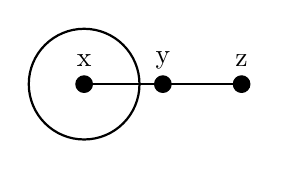
\begin{tikzpicture}

%% vertices
\draw[fill=black] (0,0) circle (3pt);
\draw (0,0.3) node{x};
\draw[fill=black] (1,0) circle (3pt);
\draw (1,0.3) node{y};
\draw[fill=black] (2,0) circle (3pt);
\draw (2,0.3) node{z};
%%% edges

\draw[thick] (0,0) circle (20pt);
\draw[thick] (0,0) -- (1,0)-- (2,0);

\end{tikzpicture}  
  
\end{subfigure}%
\begin{subfigure}{.5\textwidth}
  \centering
  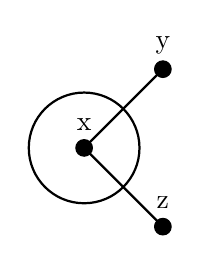
\begin{tikzpicture}

%% vertices
\draw[fill=black] (0,0) circle (3pt);
\draw (0,0.3) node{x};
\draw[fill=black] (1,1) circle (3pt);
\draw (1,1.3) node{y};
\draw[fill=black] (1,-1) circle (3pt);
\draw (1,-0.7) node{z};
%%% edges

\draw[thick] (0,0) circle (20pt);
\draw[thick] (0,0) -- (1,1);
\draw[thick] (0,0) -- (1,-1);

\end{tikzpicture}
  
\end{subfigure}

\caption{Tail and Horns. Tail is an induced path on 3 vertices, $\deg(z)=1$, $\deg(y)=2$. Horns is an induced path on 3 vertices, $\deg(z)=\deg(y)=1$.}
\label{fig:hornstail}
\end{figure}

If the tree has tail, Alice asks one color $\alpha$ for $y$ and one color $\beta$ for $z$. If $\alpha = \beta$, Alice colours the rest of the tree by induction hypothesis using $\lfloor {\frac{3(n-2)}{2}} \rfloor$ questions at most. We denote the colour of $x$ as $\gamma$. If $\gamma = \alpha = \beta$, Alice request one more colour for $y$. If $\gamma \neq \alpha = \beta$, Alice request additional colour for $z$. Now there is a colouring of the tree and there was at most $$2+\lfloor {\frac{3(n-2)}{2}} \rfloor+1=\lfloor {\frac{3n}{2}} \rfloor$$ questions by Alice.

If $\alpha \neq \beta$, by induction hypothesis and Lemma \ref{thm:difcolor} Alice can colour the rest of the tree with
$$2+\lfloor {\frac{3(n-2)}{2}} \rfloor+1=\lfloor {\frac{3n}{2}} \rfloor$$
questions and ensure that the colour of the vertex $x$ will differ from $\alpha$. We have a proper colouring.

The case when the tree has horns is similar. Alice asks one color $\alpha$ for $y$ and one color $\beta$ for $z$. If $\alpha \neq \beta$, Alice colours the rest of the tree by induction hypothesis. We denote the colour of $x$ as $\gamma$. If $\gamma = \alpha \neq \beta$, Alice request one more colour for $y$. If $\gamma = \beta \neq \alpha$, Alice request additional colour for $z$.

If $\alpha = \beta$, by induction hypothesis and Lemma \ref{thm:difcolor} Alice can colour the rest of the tree with $\lfloor {\frac{3n}{2}} \rfloor$ questions and ensure that the colour of the vertex $x$ will differ from $\alpha = \beta$.\end{pf}

\section{Joins of Graphs}


\begin{defn}
Let $G=(V,E)$ be a graph, $A\subset V$ set of vertices and $f$ a choice function for G. We say that $A$ is \emph{$f$-separable} in $G$ if for every $u,v\in A$ and every path $P$ from $u$ to $v$ there is $x\in P,\, x\neq u,v$ such that $f(x)=1$. We call vertex $x$ with $f(x)=1$ a \emph{frontier vertex}. 

We say that $A$ is \emph{separable} in $G$ if there is a choice function $f$ such that $A$ is $f$-separable.
\end{defn}


We need to introduce some temporary notation. Given a graph $G$, a vertex $v\in V(G)$, a choice function $f$ for $G$, an $f$-list assignment $L$, we define
$$ C(L, v) = \{c(v)\,|\, c \text{ is an } L\text{-colouring of } G\}.$$
We say that \emph{$v$ admits $k$ colours with $f$}, if for every $f$-list assignment $L$ we have $|C(L, v)| \geq k$.

\begin{lem}\label{lem:barvy1}
Let $G=(V,E)$ be a graph, $v \in V$, $k\in \mathbb{N}$, $h$ a choice function for $G$. Define choice function $f$ for $G$ as $f(u)=h(u)$ for $u\in V\setminus \{v\}$ and $f(v)=h(v)+k$. Then $v$ admits $k+1$ colours with $f$.
\end{lem} 

\begin{pf}
Suppose for some $f$-list assignment $L$ we have $|C(L,v)|\leq k$. We can remove colours $C(L,v)$ from the colour list $L(v)$ and obtain a $h$-list assignment $L'$ with no proper $L'$-colouring, a contradiction.
\end{pf}

\begin{lem}\label{lem:barvy2}
Let $G=(V,E)$ be a graph, $f$ a choice function for the graph $G$, $\{v_1, v_2, \ldots, v_k\}\subset V$ set of $f$-separable vertices and $L$ an $f$-list assignment. Then for every $\alpha_1 \in C(L,v_1)$, $\alpha_2 \in C(L,v_2)$, \ldots, $\alpha_k \in C(L,v_k)$ there is an $L$-colouring $c$, such that $c(v_1)=\alpha_1$, $c(v_2)=\alpha_2$, \ldots, $c(v_k)=\alpha_k$.
\end{lem} 

\begin{pf}
There are certainly $L$-colourings $c_1, c_2, \ldots, c_k$, such that $c_1(v_1)=\alpha_1$, $c_2(v_2)=\alpha_2$, $\ldots$, $c_k(v_k)=\alpha_k$ and for every frontier vertex $v\in V$ we have $c_1(v)=c_2(v)=\ldots=c_k(v)$. We can observe that frontier vertices fraction graph into separate blocks, each vertex $v_1,v_2, \ldots, v_k$ in different block, and that they do not transfer information about colouring of the adjacent blocks. So we can combine colourings $c_1, c_2, \ldots, c_k$ into a single colouring $c$ with required property.
\end{pf}



\begin{thm}\label{thm:joins}
Let $G,H$ be graphs, $P = V(G)\cap V(H)$. If $P$ is separable in $H$, then
\begin{align*}
\iscn(G \cup H) &\leq \iscn(G) + \scn(H) - |P|, \\
\scn(G \cup H) &\leq \scn(G) + \scn(H) - |P|.
\end{align*}
\end{thm}

\begin{pf}
We will first prove the second inequality. Let $h$ be a minimal choice function for $H$ such that $P$ is $h$-separable and $g$ a minimal choice function for $G$. Lets define choice function $f$ for $G\cup H$ as
$$
f(v) = \begin{cases}
g(v) & \text{ if } v\in G\setminus P \\
h(v) & \text{ if } v\in H\setminus P \\
g(v)+h(v)-1 & \text{ if } v\in P
\end{cases}.$$

The size of $f$ is $\scn(G) + \scn(H) - |P|$. For every $f$-list assignment $L$ we can clearly find a $L$-colouring of $H$. By Lemma~\ref{lem:barvy1} we see that every vertex $v\in P$ admits $g(v)$ colours with $f$ and by Lemma~\ref{lem:barvy2} we know we can use any combination of the colours on vertices in $P$. Thus among these available colours there must be a proper colouring of $G$, thus $G \cup H$.

Now we prove the first inequality. Alice starts asking exactly $h(v)$ colours for each vertex of $H$ obtaining a proper colouring of $H$. Then Alice applies her strategy for $G$. She needs only $\iscn(G)-|P|$ rounds for the second part because she already asked once for every vertex in $P$. So the strategy has length $\scn(H) + (\iscn(G)-|P|)$. 

We observe that every time Alice asks for a vertex $v$ in $P$ during the second part, it will create new colouring of $H$ with new colour for $v$ as in Lemma~\ref{lem:barvy1}. Although the new colour is not necessarily the last one added by Bob, Alice acts as it was. Again, those colours on $P$ can be arbitrarily combined by Lemma~\ref{lem:barvy2}, so Alice's strategy leads to a proper colouring of $G\cup H$.
\end{pf}

If we combine Theorem~\ref{thm:bbbd} and Theorem~\ref{thm:joins} we get the following corollary.

\begin{cor}
Conjecture~\ref{conjecture} holds if and only if it holds for every 2-connected graph.
\end{cor}

\begin{proof}
One implication is trivial. We suppose the conjecture holds for every 2-connected graph. Let $G$ be arbitrarily graph composed of two blocks $G_1, G_2$ (the general result can be easily achieved by induction). If $\iscn(G_1)<\scn(G_1)$, then using Theorem~\ref{thm:joins} and Theorem~\ref{thm:bbbd} we have $$\iscn(G)\leq \iscn(G_1)+\scn(G_2)-1 < \scn(G_1)+\scn(G_2)-1 = \scn(G).$$

If $\iscn(G_1) = \scn(G_1)$ and $\iscn(G_2) = \scn(G_2)$ then by assumption $G_1, G_2$ are cliques. We show by induction on number of vertices that the interactive sum choice number of union of cliques having one vertex in common is strictly smaller then it's sum choice number.

Let $G_1 = K_n$ and $G_2 = K_m$. We know that \begin{align*}
\scn(K_n \cup K_m) &= \scn(K_n) + \scn(K_m) -1 = \\
&=|V(K_n)|+|E(K_n)|+|V(K_m)|+|E(K_m)|-1 = \\
&= {n+1 \choose 2} + {m+1 \choose 2} -1,
\end{align*}

and we show that $$\iscn(K_n \cup K_m) \leq {n+1 \choose 2} + {m+1 \choose 2} - 2.$$

If $n=m=2$, the proposition holds. WLOG let $n\geq 3$. Pick an arbitrary vertex $v$ from $K_n$. We notice there is $n-1$ neighbours of $v$. By induction hypothesis Alice can colour graph $G\setminus\{v\}$ in $${n \choose 2} + {m+1 \choose 2} - 2$$ rounds. Then Alice asks additional $n$ colours for vertex $v$. Since $v$ has more colours than neighbours, there must be proper colouring of $G$. Thus Alice can colour $G$ in \begin{align*}
\iscn(G) &\leq {n \choose 2} + {m+1 \choose 2} - 2 + n = \\
&= {n+1 \choose 2} + {m+1 \choose 2} - 2
\end{align*}
rounds.
\end{proof}


\section{Sc-greedy Graphs}

We show in this section that any sc-greedy graph satisfies Conjecture~\ref{conjecture}. Bonamy and Meeks concluded the same from the following theorem.
\begin{othm}[Theorem 3.2 in \cite{iscn}]
Let $G$ be a connected graph on $n \geq 3$ vertices. If $G$ is sc-greedy, then
$$\iscn(G) \leq \scn(G) - \frac{n-\omega(G)}{2}.$$
\end{othm} 

\begin{figure}[h]
\centering
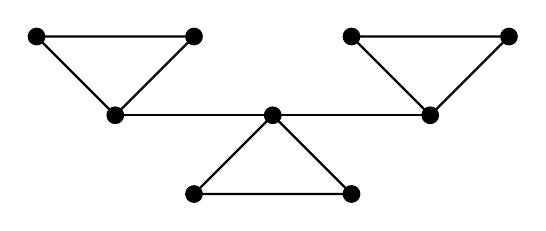
\begin{tikzpicture}

%% vertices
\draw[fill=black] (0,1) circle (3pt);
\draw[fill=black] (1,0) circle (3pt);
\draw[fill=black] (2,1) circle (3pt);
\draw[fill=black] (2,-1) circle (3pt);
\draw[fill=black] (3,0) circle (3pt);
\draw[fill=black] (4,-1) circle (3pt);
\draw[fill=black] (4,1) circle (3pt);
\draw[fill=black] (5,0) circle (3pt);
\draw[fill=black] (6,1) circle (3pt);
%%% edges

\draw[thick] (1,0) -- (3,0) -- (5,0);
\draw[thick] (0,1) -- (1,0) -- (2,1) -- (0,1);
\draw[thick] (2,-1) -- (4,-1) -- (3,0) -- (2,-1);
\draw[thick] (4,1) -- (5,0) -- (6,1) -- (4,1);

\end{tikzpicture}
\caption{A counterexample to Theorem~3.2 in \cite{iscn}.}
\label{fig:counterexample}
\end{figure}

Unfortunately the theorem is false, see a counterexample $G$ in Figure~\ref{fig:counterexample}. We have $\iscn(G) \geq 3\cdot\iscn(K_3) = 18$ and since $G$ is sc-greedy (Theorem~\ref{thm:bbbd}) we have $$\scn(G) - \frac{n-\omega(G)}{2} = 9 + 11 - \frac{9-3}{2} = 17.$$

The rest of their article remains unaffected, the theorem was not essential.

\begin{prop}\label{thm:scg}
Conjecture~\ref{conjecture} holds for all sc-greedy graphs.
\end{prop}

\begin{pf}
Every graph can be constructed from an induced subgraph by adding stars. Let $G=(V,E)$ be an incomplete graph. Then there is an induced path on 3 vertices. We denote the path as $H$. We have $\iscn(H)=4$, $|V(H)| + |E(H)| = 5$. We reconstruct $G$ from $H$ by adding stars. At each step, by denote current subghraph as $H_i$, that is $H_0=H,\ldots,H_n=G$. By Theorem~\ref{thm:joins} we have \begin{align*}
|V(H_{i+1})| &+ |E(H_{i+1})| - \iscn(H_{i+1}) = \\
&= |V(H_{i})| + |E(H_{i})| + k + 1 - \iscn(H_i \cup K_{1,k}) = \\
&\geq |V(H_{i})| + |E(H_{i})| + k + 1 - (\iscn(H_i) + \scn(K_{1,k}) - k) = \\
&= |V(H_{i})| + |E(H_{i})| + k + 1 - \iscn(H_i) - 2k - 1 + k = \\
&= |V(H_{i})| + |E(H_{i})| - \iscn(H_i).
\end{align*}
Thus we have
\begin{align*}
\scn(G) - \iscn(G) &= |V(G)| + |E(G)| - \iscn(G) \geq \\
	&\geq |V(H_{n-1})| + |E(H_{n-1})| - \iscn(H_{n-1}) = \\
	&\geq ... \geq \\
	&\geq |V(H_1)| + |E(H_1)| - \iscn(H_1) \geq \\
 	&\geq |V(H)| + |E(H)| - \iscn(H) = \\
 	&= 5 - 4 = 1,
\end{align*}
as required.
\end{pf}

For every graph $G$ we denote $\gb(G) = |V(G)| + |E(G)|$ (\emph{greedy bound}). Using the same technique as above we obtain a generalized version of Proposition~\ref{thm:scg}. We observe that the interactive sum choice number can be replaced by the sum choice number, we just use the other part of Theorem~\ref{thm:joins}.

\begin{thm}
For every graph $G$ and an induced subgraph $H$ we have the inequalities
\begin{align*}
\gb(H) - \iscn(H) &\leq \gb(G) - \iscn(G), \\
\gb(H) - \scn(H) &\leq \gb(G) - \scn(G).
\end{align*}
\end{thm}

\section{Fan Graphs}

\emph{A fan graph} $F_n$ is a path on $n$ vertices together with a vertex $v_0$ connected with every vertex of the path, see Figure~\ref{fig:fan}.

Heinold showed that fan graphs are not sc-greedy in general, although the smallest counterexample is $F_{10}$ \cite{heinold2006}.

\begin{figure}[h]
\centering
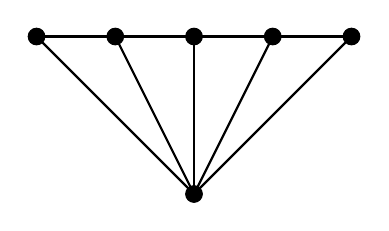
\begin{tikzpicture}

%% vertices
\draw[fill=black] (0,0) circle (3pt);
\draw[fill=black] (1,0) circle (3pt);
\draw[fill=black] (2,0) circle (3pt);
\draw[fill=black] (3,0) circle (3pt);
\draw[fill=black] (4,0) circle (3pt);
\draw[fill=black] (2,-2) circle (3pt);
%%% edges

\draw[thick] (0,0) -- (1,0) -- (2,0) -- (3,0) -- (4,0);
\draw[thick] (2,-2) -- (0,0);
\draw[thick] (2,-2) -- (1,0);
\draw[thick] (2,-2) -- (2,0);
\draw[thick] (2,-2) -- (3,0);
\draw[thick] (2,-2) -- (4,0);

\end{tikzpicture}
\caption{Fan graph $F_5$}
\label{fig:fan}
\end{figure}



\begin{prop}
Conjecture~\ref{conjecture} holds for all fan graphs $F_n$.
\end{prop}


\begin{pf}
It is sufficient to prove the proposition for $n\geq 10$, as fan graphs are sc-greedy for $n< 10$ and the conjecture holds due the Proposition~\ref{thm:scg} for $n< 10$.

Given a fan graph $F_n$, denote the vertices on the path as $v_1, v_2, \ldots, v_n$ and the distinct vertex as $v_0$. We compute an upper bound on the interactive sum choice number. We have 
$$\iscn(F_n) \leq \lfloor{\frac{3n}{2}}\rfloor + n + 1 = \lfloor{\frac{5n+2}{2}}\rfloor,$$ since Alice has a strategy of length $\lfloor{\frac{3n}{2}}\rfloor$ for colouring of the path (Proposition~\ref{thm:odhady}) and additional $n+1$ colors for $v_0$ are sufficient to find a colouring of $F_n$.

Now we consider a subgraph $E_n \subseteq F_n$, where we remove all edges between $v_{2k}$ and $v_{2k+1}$, $2\leq k < n/2$ (see Figure~\ref{fig:fan2}). We have $\scn(F_n) \geq \scn(E_n)$, so we have to find a lower bound on $\scn(E_n)$. 

\begin{figure}[h]
\centering
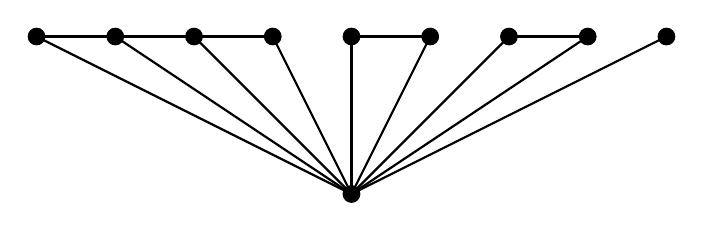
\begin{tikzpicture}

%% vertices
\draw[fill=black] (0,0) circle (3pt);
\draw[fill=black] (1,0) circle (3pt);
\draw[fill=black] (2,0) circle (3pt);
\draw[fill=black] (3,0) circle (3pt);
\draw[fill=black] (4,0) circle (3pt);
\draw[fill=black] (5,0) circle (3pt);
\draw[fill=black] (6,0) circle (3pt);
\draw[fill=black] (7,0) circle (3pt);
\draw[fill=black] (8,0) circle (3pt);
\draw[fill=black] (4,-2) circle (3pt);
%%% edges

\draw[thick] (0,0) -- (1,0) -- (2,0) -- (3,0);
\draw[thick] (4,0) -- (5,0);
\draw[thick] (6,0) -- (7,0);
\draw[thick] (4,-2) -- (0,0);
\draw[thick] (4,-2) -- (1,0);
\draw[thick] (4,-2) -- (2,0);
\draw[thick] (4,-2) -- (3,0);
\draw[thick] (4,-2) -- (4,0);
\draw[thick] (4,-2) -- (5,0);
\draw[thick] (4,-2) -- (6,0);
\draw[thick] (4,-2) -- (7,0);
\draw[thick] (4,-2) -- (8,0);

\end{tikzpicture}
\caption{Subgraph $E_9$}
\label{fig:fan2}
\end{figure}

The graph $E_n$ is a block graph, we denote the blocks from left to right as $G_1, G_2, \ldots, G_k$, $k=\lfloor{(n-1)/2}\rfloor$. All blocks are sc-greedy, $\scn(G_1) = 12$, $\scn(G_i)= 6, 1<i<k$ and $\scn(G_k)\geq 3$. By Theorem~\ref{thm:bbbd} we have
\begin{align*}
\scn(E_n) &= \scn(G_1) + (k-2)\scn(G_i) + \scn(G_k) - k + 1 \geq \\
	&\geq 16 + 6\lfloor{\frac{n-1}{2}}\rfloor - \lfloor{\frac{n-1}{2}}\rfloor = \\
	&= 16 + 5\lfloor{\frac{n-1}{2}}\rfloor = \\
	&= \lfloor{16 + 5\frac{n-1}{2}}\rfloor = \\
	&= \lfloor{\frac{5n-5+32}{2}}\rfloor = \\ 
	&= \lfloor{\frac{5n+3}{2}}\rfloor + 12 > \iscn(F_n).
\end{align*}
\end{pf}




\section{Ear Decomposition}

Well-known ear decomposition lemma states that every 2-connected graph can be obtained from a cycle by adding ears. We denote $G+P_n$ adding the ear $P_n$ to the graph $G$, that is joining by the endpoints of the path. The lemma led us to the following propositions.

\begin{prop}
Let $G$ be a graph, $P_n$ a path on $n\geq 3$ vertices. Then 
\begin{align*}
\iscn(G+P_n) &\leq \iscn(G)+\scn(P_n)-2, \\
\iscn(G+P_n) &\leq \iscn(G)+\iscn(P_n)-1.
\end{align*}
\end{prop}

\begin{pf}
The first inequality is a trivial application of Theorem~\ref{thm:joins}. We prove the second inequality. Denote the vertices of the path $v_1, \ldots, v_n$. Alice colour $G$ with $\iscn(G)$ questions. Then she finds a colouring of the interior $v_2, \ldots, v_{n-1}$ of the path, such that the colour of $v_2$ differs from $v_1$ and the colour of $v_{n-1}$ differs from $v_n$. By Lemma~\ref{thm:difcolor}, this can be done in $$\iscn(P_{n-2})+2 = \lfloor{\frac{3(n-2)}{2}}\rfloor+2 = \lfloor{\frac{3n}{2}}\rfloor-1 = \iscn(P_n)-1$$ rounds.
\end{pf}

\begin{prop}
Let $G$ be a graph, $P_n$ a path on $n\geq 3$ vertices. Then 
$$\scn(G+P_n) \geq \scn(G)+\scn(P_n)-3.$$
\end{prop}

\begin{pf}
Denote the vertices of the path $v_1, \ldots, v_n$. We remove the edge $v_1v_2$ from $G+P_n$ forming a subgraph $H$. By Theorem~\ref{thm:bbbd} we have 
\begin{align*}
\scn(G+P_n) \geq \scn(H) &= \scn(G) + \scn(P_{n-1}) - 1 = \\
 &= \scn(G)+\scn(P_n)-3.
\end{align*}
\end{pf}

\begin{prop}
Conjecture~\ref{conjecture} holds for every 2-connected graph, which can be obtained from a cycle by adding ears on 5 or more vertices .
\end{prop}
\begin{pf}
For $n\geq 5$ we have 
\begin{align*}
\lfloor{\frac{3n}{2}}\rfloor &\leq 2n-3 \\
\lfloor{\frac{3n}{2}}\rfloor -1 &\leq 2n -1 -3 \\
\iscn(P_n)-1 &\leq \scn(P_n)-3.
\end{align*}
Thus if $\iscn(G) < \scn(G)$, then
\begin{align*}
\iscn(G+P_n) &\leq \iscn(G)+\iscn(P_n)-1 < \\
			&< \scn(G)+\scn(P_n)-3 \leq \scn(G+P_n). \\
\end{align*}
If we start with a cycle $C$ on 4 or more vertices, we have $\iscn(C) < \scn(C)$ and the proposition follows by the induction step above. The case when we start with a 3-cycle have to be analysed separately, but it can be easily shown that $\iscn(G) < \scn(G)$ for $G=C_3+P_n$, $n\geq 4$ by a simple case analysis.
\end{pf}

\begin{prop}
Let $G=H+P_n$, $n\geq 7$. Then $\iscn(G) < \scn(G)$.
\end{prop}

\begin{pf}
For $n\geq 7$ we have 
\begin{align*}
\lfloor{\frac{3n}{2}}\rfloor &< 2n-3 \\
\lfloor{\frac{3n}{2}}\rfloor -1 &< 2n -1 -3 \\
\iscn(P_n)-1 &< \scn(P_n)-3.
\end{align*}
Thus
\begin{align*}
\iscn(H+P_n) &\leq \iscn(H) + \iscn(P_n) - 1 = \\
 &\leq \scn(H) + \iscn(P_n) - 1 < \\
 &< \scn(H) + \scn(P_n) - 3 \leq \scn(H+P_n).
\end{align*}
\end{pf}

\section{Concluding Remarks}

We have studied the interactive sum choice number introduced by Bonamy and Meeks \cite{iscn}. We have created tools giving an upper bound on the interactive sum choice number of an union of graphs and we have given several applications of the tools. 


Mainly, we have concluded that it is sufficient to prove Conjecture~\ref{conjecture} for 2-connected graphs and we proved Conjecture~\ref{conjecture} for fan graphs and for sc-greedy graphs.


\begin{figure}[h]
\centering
\begin{subfigure}{.5\textwidth}
  \centering
  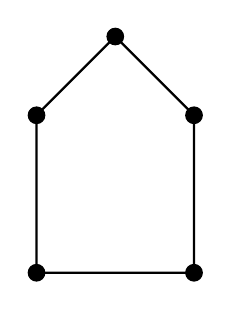
\begin{tikzpicture}

%% vertices
\draw[fill=black] (0,0) circle (3pt);
\draw[fill=black] (2,0) circle (3pt);
\draw[fill=black] (2,2) circle (3pt);
\draw[fill=black] (1,3) circle (3pt);
\draw[fill=black] (0,2) circle (3pt);
%%% edges

\draw[thick] (0,0) -- (2,0) -- (2,2)-- (1,3)--(0,2)--(0,0);

\end{tikzpicture} 
  
\end{subfigure}%
\begin{subfigure}{.5\textwidth}
  \centering
  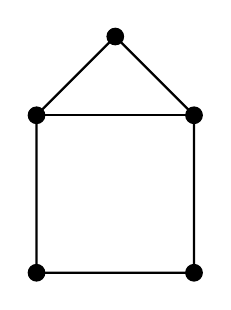
\begin{tikzpicture}

%% vertices
\draw[fill=black] (0,0) circle (3pt);
\draw[fill=black] (2,0) circle (3pt);
\draw[fill=black] (2,2) circle (3pt);
\draw[fill=black] (1,3) circle (3pt);
\draw[fill=black] (0,2) circle (3pt);
%%% edges

\draw[thick] (0,0) -- (2,0) -- (2,2)-- (1,3)--(0,2)--(0,0);
\draw[thick] (0,2) -- (2,2);

\end{tikzpicture}
  
\end{subfigure}

\caption{Cycle $C_5$ and “house" graph $H$}
\label{fig:houseg}
\end{figure}


We felt enthusiastic about the use of the ear decomposition lemma and we have given some partial results for graphs created by adding ears. The biggest problem of this approach may be adding ears on 2 vertices (that is adding edges), since those are not separable and Theorem~\ref{thm:joins} cannot be used. Furthermore adding an edge have unpredictable effect on the interactive sum choice number. Sometimes it grows really high \cite{iscn}, sometimes it remains the same. A concrete example is the cycle $C_5$ and the “house" graph $H$ (see Figure~\ref{fig:houseg}), for both $\iscn(C_5) = \iscn(H) = 9$. 



\begin{thebibliography}{99}
\bibitem{heinold2011}
  Brian Heinold 
  (2011),
  \textit{A few sum list coloring facts},
  \url{https://www.brianheinold.net/articles/slc_stuff.pdf},
  [Online; accessed 22-February-2018]
  
\bibitem{heinold2006}
  Brian Heinold
  (2006),
  \textit{Sum List Coloring and Choosability},
  dissertation,
  Lehigh University
  
\bibitem{iscn}
  Marthe Bonamy, Kitty Meeks
  (2017),
  \textit{The Interactive Sum Choice Number of Graphs},
  {\tt \href{https://arxiv.org/abs/1703.05380v2}{arXiv:1703.05380v2 [cs.DM]}}

\end{thebibliography}






\end{document}